
% Beamer document class
\documentclass[xcolor=dvipsnames]{beamer}
% packages
\usepackage[utf8]{inputenc}
%\usepackage{latexsym}
\usepackage{graphicx}
\usepackage{mathptmx}
\usepackage{amsmath}
\usepackage{amsfonts}
\usepackage{amssymb}
\usepackage{amsbsy}
\usepackage{amsthm}
\usepackage{algorithmic}

% Get checkmark logo
\usepackage{pifont}
\newcommand{\cmark}{\ding{51}}
\newcommand{\xmark}{\ding{55}}

% Set VT theme
\usepackage{pgf} % For image/line placement.
% Set a minimal theme with maroon background colors
\setbeamercolor*{palette tertiary}{bg=Maroon}
\setbeamercolor{frametitle}{fg=Black}
\setbeamercolor{section in toc}{fg=Black}
\setbeamercolor{subsection in toc}{fg=Black}
\setbeamercolor{title}{fg=Black}
\setbeamercolor{item}{fg=Black}
\setbeamercolor{block title}{fg=Black,bg=Maroon!20}
\setbeamercolor{caption name}{fg=Black}
% Set the math fonts
\usefonttheme[onlymath]{serif}
\DeclareMathAlphabet{\mathcal}{OMS}{cmsy}{m}{n}
% Create a maroon hline under the frame title
\newcommand{\VThline}{%
\raisebox{-12mm}[0pt][0pt]{%
\begin{pgfpicture}{0mm}{0mm}{0mm}{0mm}
\pgfsetlinewidth{0.28mm}
\color{Maroon}
\pgfline{\pgfpoint{-3mm}{1mm}}{\pgfpoint{10.8cm}{1mm}}
\end{pgfpicture}}}
\setbeamertemplate{headline}{\VThline}
% Add the VT logo to the top right
\newcommand{\VTlogo}{
\vspace*{0.4cm}\hspace*{-3cm}
{
\includegraphics[height=0.5cm]{VPIlogo.png}}}
\setbeamertemplate{sidebar canvas right}{\VTlogo}
% Add page numbers
\setbeamertemplate{footline}[frame number]

% Title Information
\title{Algorithms and Software for Delaunay Interpolation and
Multiobjective Optimization}
\date{\today}
\author{Tyler H. Chang}
\institute{Dept. of Computer Science \\
Virginia Polytechnic Institute and State University}

\begin{document}

% Make title frame with footnote
\begin{frame}[plain] % plain removes the formatting
\vfill
\titlepage
\vfil % No skip above the logo. If logo is removed, change to \vfill
% Adds logo to bottom of the title page
\centerline{
\includegraphics[height=0.5cm]{VPIlogo.png}}
\end{frame}

% About slides
\begin{frame}{About me}
\begin{itemize}
\item Ph.D. candidate at Virginia Tech
\item Advisor: Dr.\ Layne Watson
\item Interests: Analysis! (Numerical, Functional, Stochastic)
\item Skills: Algorithms, Parallel Computing, Low-Level Languages
\item Application areas: Data Science, Engineering Design, Quantum Computing
\end{itemize}
\end{frame}
% Make ToC
\begin{frame}{Table of Contents}
\tableofcontents
\end{frame}
% Section on Delaunay triangulations
\section{DELAUNAYSPARSE package}
\subsection{The Delaunay interpolation problem}
% What is Delaunay triangulation
\begin{frame}{About Delaunay Triangulations}
\begin{itemize}
\item The {\it Delaunay triangulation} is an unstructured simplicial mesh
defined by an arbitrary vertex set $P = \{p_1, \ldots, p_n\} \subset \mathbb{R}^d$
\item The defining property of the Delaunay triangulation $DT(P)$ is that
for every simplex $S \in DT(P)$, the circumball $B_S$ must have
empty intersection with $P$: $B_S \cap P = \emptyset$.
\end{itemize}
\begin{center}
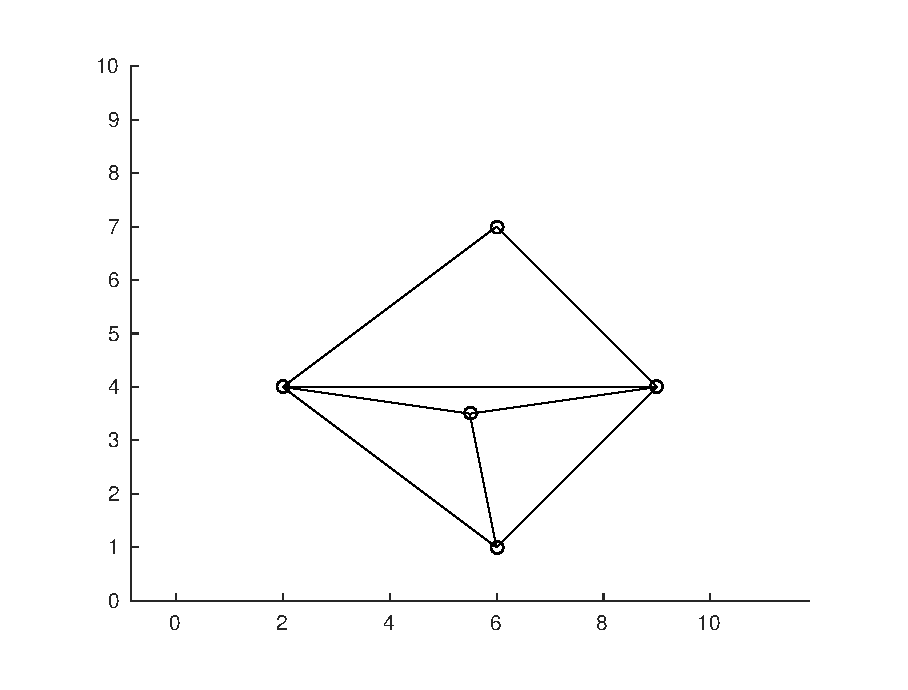
\includegraphics[width=0.45\textwidth]{triangleplane.eps}{\color{Red} \xmark}
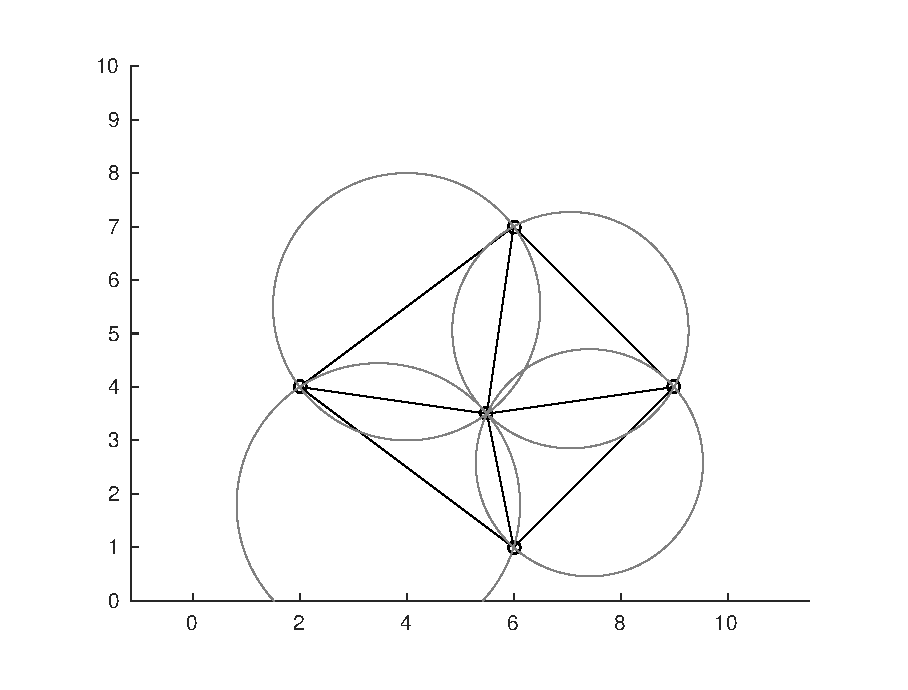
\includegraphics[width=0.45\textwidth]{delaunayplane.eps}{\color{Green} \cmark}
\end{center}
\end{frame}
% Brief applications of Delaunay
\begin{frame}{Applications of Delaunay Triangulations}
\begin{columns}
\begin{column}{.48\textwidth}
\begin{itemize}
\item Interpolation mesh for
\begin{itemize}
\item Finite element method,
\item data science,
\item GIS, and
\item computer graphics
\end{itemize}
\item Delaunay graph
\end{itemize}
\end{column}
\begin{column}{.48\textwidth}
\hbox{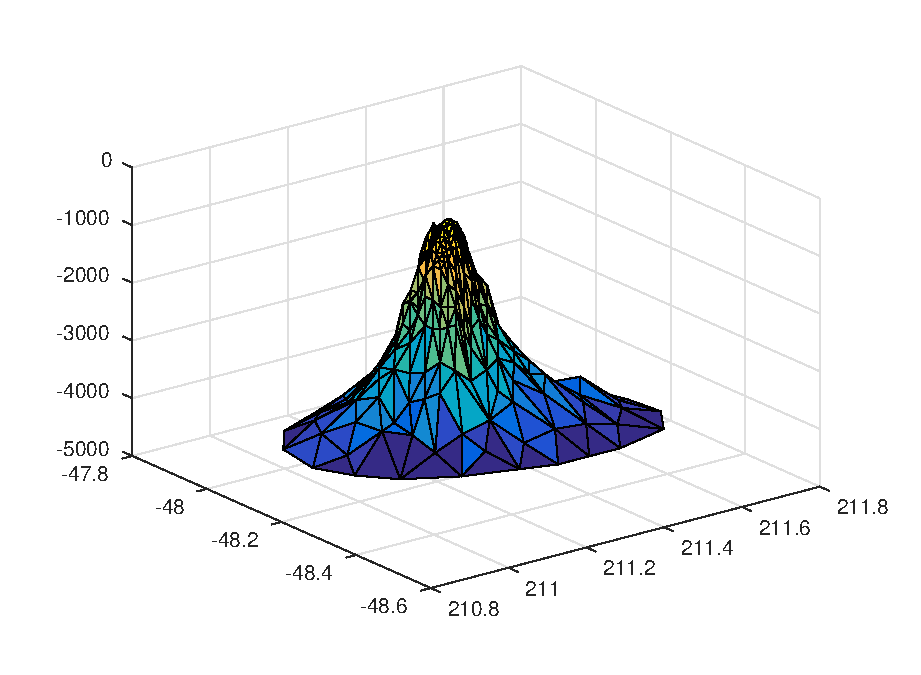
\includegraphics[width=.9\textwidth]{seamount.eps}}
\end{column}
\end{columns}
\bigskip
\pause
{\bf Piecewise linear interpolation:}
Let $f : \mathbb{R}^d \rightarrow \mathbb{R}$, and let $q \in S \in DT(P)$.
$S$ has vertex set $\{s_1, \ldots, s_{d+1}\}$ and there exist convex weights
$\{w_1, \ldots, w_{d+1}\}$ such that $q = \sum_{i=1}^{d+1} w_i s_i$.
$$
{\hat f}_{DT}(q) = \sum_{i=1}^{d+1} w_i f(s_i).
$$
\end{frame}
% Interpolation problem
\begin{frame}{Delaunay interpolation}
\textbf{Problem}: the size of the Delaunay triangulation is
$\mathcal{O}\left(n^{\lceil d/2 \rceil}\right)$
\begin{itemize}
\item For $d > 4$, this is expensive!
\item For $d > 8$, this is not scalable!
\end{itemize}
\medskip
\textbf{Observation:}
For interpolation, we only need the
vertices ($\{s_1, \ldots, s_{d+1}\}$) of $S \in DT(P)$ such that $q\in S$
$$
{\hat f}_{DT}(q) = \sum_{i=1}^{d+1} w_i\text{~}f(s_i).
$$
\medskip
\textbf{Question:}
Can we find $S$ containing $q$ in polynomial time (without computing the whole mesh)?
\end{frame}
% Algorithm description
\subsection{Algorithm for Delaunay interpolation}
% Algorithm for computing the Delaunay interpolant
\begin{frame}{Algorithm outline}
\begin{itemize}
\item Grow an initial simplex (greedy algorithm)
\item ``Flip'' accross a facet from which $q$ is visible
\item This ``visibility walk'' converges to $q$ in $k$ steps
(Edelsbrunner's acyclicity theorem)
\end{itemize}
Full algorithm published in
{\small \it Tyler H. Chang, et al. 
``A polynomial time algorithm for multivariate interpolation in arbitrary
dimension via the Delaunay triangulation.''
In the ACMSE 2018 Conf.}\\
\medskip
{\bf Overall complexity:} $\mathcal{O}(nd^2 k)$
\end{frame}
% Implementation description
\subsection{Serial implementation}
% DELAUNAYSPARSE
\begin{frame}{DELAUNAYSPARSE Package}
Standalone software package {\tt DELAUNAYSPARSE}:
\begin{itemize}
\item Robust against degeneracy
\item Runs in $\mathcal{O}(k m n d^2)$ time, where $k$ is the
number of ``flips'', $n$ is the numer of data points, $m$ is the number of
interpolation points, and $d$ is the input dimension
\item Typically, $k \approx \mathcal{O}(d\log d)$
\item Parallel and serial implementations
\end{itemize}
Under review:
{\small \it Tyler H. Chang, et al.
``Algorithm XXX: DELAUNAYSPARSE: Interpolation via a sparse subset of the
Delaunay triangulation in medium to high dimensions.''
Submitted to ACM Transactions on Mathematical Software (2019)}. 
\end{frame}
% Serial performance
\begin{frame}{Serial performance}
Runtime in seconds for interpolating a single point ($m=1$) with $n$ points
in $d$ dimensions\\
\bigskip
\medskip
\begin{tabular}{c|ccccc}
& & & $d$ & & \\
$n$ & 2 & 8 & 32 & 64 & 128 \\
\hline
100 & 0.001 & 0.004 & 0.060 & 0.820 & n/a \\
500 & 0.021 & 0.042 & 0.325 & 6.479 & 59.511 \\
2000 & 0.344 & 0.583 & 2.230 & 28.984 & 242.066 \\
8000 & 5.580 & 9.027 & 26.210 & 151.177 & 905.711 \\
16,000 & 22.086 & 35.725 & 109.448  & 386.596  & 2190.362 \\
32,000 & 82.915 & 145.115 & 421.934 & 1097.060 & slow \\
\end{tabular}
\end{frame}
% Parallel implementation
\subsection{Parallel implementation}
\begin{frame}{Parallel implementation}
\begin{itemize}
\item Level 1: loop over multiple interpolation points
\item Level 2: loop(s) over data points -- imperfect scaling
\end{itemize}
\medskip
\begin{columns}
\begin{column}{.48\textwidth}
\includegraphics[width=.95\textwidth]{d10n1000m1024.eps}
$$
d=10\text{, }n=1000\text{, }m=1024
$$
\end{column}
\begin{column}{.48\textwidth}
\includegraphics[width=.95\textwidth]{d10n10000m64.eps}
$$
d=10\text{, }n=10,000\text{, }m=64
$$
\end{column}
\end{columns}
\begin{center}
\includegraphics[width=0.44\textwidth]{d20n200m64.eps}\\
$d=20\text{, }n=200\text{, }m=64$
\end{center}
\end{frame}
% Applications
\subsection{Applications and future work}
\begin{frame}{Applications of DELAUNAYSPARSE}
\begin{columns}
\begin{column}{.48\textwidth}
\begin{itemize}
\item HPC system data interpolation
\begin{itemize}
\item Nonparametric distribution interpolation
\end{itemize}
\item Aerospace engineering -- oblique shock calculation
\begin{itemize}
\item Surrogate model to ``warm start'' calculations
\end{itemize}
\item Data science applications
\begin{itemize}
\item Comparison with neural network and support vector regressors
\end{itemize}
\end{itemize}
\end{column}
\begin{column}{.48\textwidth}
\includegraphics[width=\textwidth]{delaunay-dist-ex.pdf}
\end{column}
\end{columns}
\end{frame}
% Future work
\begin{frame}{Future work}
\begin{itemize}
\item Delaunay interpolation in an arbitrary metric space
\item Other sparse subsets, such as umbrella neighborhood\\
{\it \small Tyler H. Chang, et al. 
``Computing the umbrella neighbourhood of a vertex in the Delaunay 
triangulation and a single Voronoi cell in arbitrary dimension.''
In IEEE SoutheastCon 2018.}
\end{itemize}
\end{frame}

% Pause/reset
\begin{frame}{Pause \& Reset}
\begin{center}
{\huge
Questions about Delaunay interpolation?
}
\end{center}
\end{frame}

% VTMOP section
\section{VTMOP package}
\subsection{Background in MOPs}
% High-level MOP defn
\begin{frame}{What is a MOP?}
\begin{itemize}
\item The Multiobjective Optimization Problem (MOP) generalizes the Single
Objective (Scalar) Optimization Problem (SOP);
\item The MOP attempts to balance the tradeoff between multiple conflicting
objectives;
\item Whereas the SOP generally has a unique solution, the solution to a MOP
is a {\it set} of {\it Pareto optimal} solutions;
\end{itemize}
\begin{center}
\includegraphics[width=0.45\textwidth]{feasible_design.eps}
\includegraphics[width=0.45\textwidth]{convex_pareto.eps}
\end{center}
\end{frame}
% Pareto/efficient defn
\begin{frame}{Goals:}
\begin{center}
\begin{tabular}{|ccc|}
\hline
&&\\
&{\large Find a discrete set of approximately}&\\
&{\large nondominated objective points that}&\\
&{\large describes the Pareto front, and the}&\\
&{\large corresponding efficient designs}&\\
&&\\
\hline
\end{tabular}
\end{center}
\end{frame}
% Blackbox problems
\begin{frame}{Expensive Blackbox MOPs}
\begin{center}
{\bf Types of MOPs}\\
\smallskip
{\footnotesize
\begin{tabular}{|c|c|}
\hline
\begin{tabular}{c}
 \\
functions are ``cheap'' to evaluate\\
derivative info is available\\
\\
\end{tabular}
& 
\begin{tabular}{c}
 \\
functions are ``cheap'' to evaluate\\
no derivative info is available\\
\\
\end{tabular}\\
\hline
\begin{tabular}{c}
\\
functions are costly to evaluate\\
derivative info is available\\
\\
\end{tabular}
&
\begin{tabular}{c}
\\
functions are costly to evaluate\\
no derivative info is available\\
\\
\end{tabular}\\
\hline
\end{tabular}
}
\end{center}
\medskip
Focus on bottom right: {\bf expensive blackbox MOPs}!
\end{frame}
% Application subsection
\subsection{An application}
% VarSys problem
\begin{frame}{Motivating Example: VarSys}
\textbf{VarSys:} Managing performance variance
\begin{itemize}
\item For multiple runs of the same I/O task on the same HPC system,
we get varying throughputs
\item This presents issues for load balancing and performance guarantees
\item Needs to be balanced against other concerns such as energy consumption
and mean throughput
\item Evaluation expense: 1+ minutes to build distributions
\end{itemize}
\end{frame}
%% Common techniques
%\begin{frame}{Common techniques}
%\begin{itemize}
%\item Multiobjective Evolutionary Algorithms
%\begin{itemize}
%\item Requires many function evaluations
%\item Random by nature
%\end{itemize}
%\item Multiobjective Direct Search
%\begin{itemize}
%\item Mainly for biobjective case
%\end{itemize}
%\item Scalarization
%\begin{itemize}
%\item Reduce MOP to SOP using scalarization function
%\item Solve many scalarized subproblems
%\end{itemize}
%\end{itemize}
%\end{frame}
%% Weighted sum
%\begin{frame}{Weighted Sum Method}
%$$
%\min_{x\in\mathcal{X}}\text{ } w^T F(x) \text{, for } w \succeq \Vec{0}
%$$
%\begin{itemize}
%\item For $w > \Vec{0}$, the solution is Pareto optimal
%\item An {\it adaptive weighting scheme} is required
%\item Cannot produce solutions in nonconvex regions of Pareto front\\
%$\qquad\qquad$
%\includegraphics[width=0.5\textwidth]{nonconvex_pareto.eps}
%\end{itemize}
%\end{frame}
%% RSM
%\begin{frame}{The Response Surface Methodology}
%\begin{itemize}
%\item Do an experimental design, use design to fit ``cheap'' surrogate models,
%use surrogates to predict optimal designs
%\item Very economic for blackbox problems
%\item Useful for MOP since the models can be reused for multiple
%scalarizations
%\end{itemize}
%\end{frame}

% Main proposal section
\subsection{VTMOP algorithm}
% Introducing VTMOP solver...
\begin{frame}{VTMOP}
\texttt{VTMOP} is a Fortran 2008 blackbox MOP solver and framework,
based on an algorithm by
{ \small \it Shubhangi Deshpande, et al.
``Multiobjective optimization using an adaptive weighting scheme.''
Optimization Methods and Software 31.1 (2016): 110-133.}\\
\medskip
{\tt VTMOP} is meant to be flexible, scalable, portable, robust, and
efficient for solving expensive blackbox MOPs\\
\medskip
Combines adaptive weighting scheme, response surface modeling, and trust
region methods
\end{frame}
% Describing Shubhangi's algorithm
\begin{frame}{The Algorithm Outline}
\begin{center}
\includegraphics[width=0.95\textwidth]{algorithm-chart.pdf}
\end{center}
\end{frame}
% Describing Shubhangi's algorithm
\begin{frame}{Key component}
\begin{center}
\includegraphics[width=0.95\textwidth]{isolated-chart.png}
\end{center}
\end{frame}
% Identifying an isolated point
\begin{frame}{Identifying an Isolated Point}
Let $P^{(k)}$ be the $k$th set of nondominated objective points
$P^{(k)} = \{X^{(1,k)}, \ldots, X^{(N_k,k)}\} $.
\medskip
Define the projected set 
$$
H^{(k)} = \left\{ \left(\frac{X^{(n,k)}_1}{X^{(n,k)}_p}, \ldots,
\frac{X^{(n,k)}_{p-1}}{X^{(n,k)}_p}\right) \quad\bigg|\quad
n = 1, \ldots, N_k\right\}
$$
The most isolated point is identified by considering the average
Euclidean distance to all neighbors in the Delaunay graph of $H^{(k)}$\\
\begin{center}
\includegraphics[width=.5\textwidth]{del-nbhd.png}\\
{\it Image from Wikipedia}
\end{center}
\end{frame}
% Getting the Delaunay graph
\begin{frame}{Getting the Delaunay Graph}
\textbf{Compute the Delaunay neighborhood} of $X^{(1,k)}$, $\ldots$,
$X^{(N_k,k)}$ with respect to the projected set $H^{(k)}$.\\
\medskip
\begin{itemize}
\item Only need the Delaunay graph $G_{DT}$
\item Number of connections in $G_{DT}$ is upper bounded by $N_k(N_k-1)/2$
\item Can recover $G_{DT}$ by interpolating the midpoint between each pair
of points in $H^{(k)}$
\item Using {\tt DELAUNAYSPARSE}, requires
$\mathcal{O}(N_k^3 p^3 \log p)$ time
\end{itemize}
\end{frame}
% Section on Parallel versions
\subsection{Parallel implementation}
% How to use parallelism
\begin{frame}{Parallel implementations}
Focus on achieving parallel function evaluations:
\begin{itemize}
\item One ``unmodified'' implementation -- distributes function evaluations
that can be done asynchronously without changing the original algorithm
\item The {\tt libEnsemble} implementaion -- integrates with Argonne's
{\tt libEnsemble} library (part of the Exascale Computing Project) to
achieve increased levels of concurrency
\begin{itemize}
\item Required significant modification to the
underlying algorithm
\end{itemize}
\end{itemize}
{\it \small
Tyler H. Chang, et al.
``Managing computationally expensive blackbox multiobjective optimization
problems with libEnsemble.''
Submitted to SpringSim 2020, 28th HPC Symposium.
}
\end{frame}
% Test functions
\begin{frame}{Benchmark problems}
\begin{columns}
\begin{column}{.48\textwidth}
\begin{itemize}
\item $F_{c}(x) = (\|x - e_1\|_2^2, \ldots, \|x - e_p\|_2^2)$
\item Convex Pareto front $\Rightarrow$ ``easier'' problem
\end{itemize}
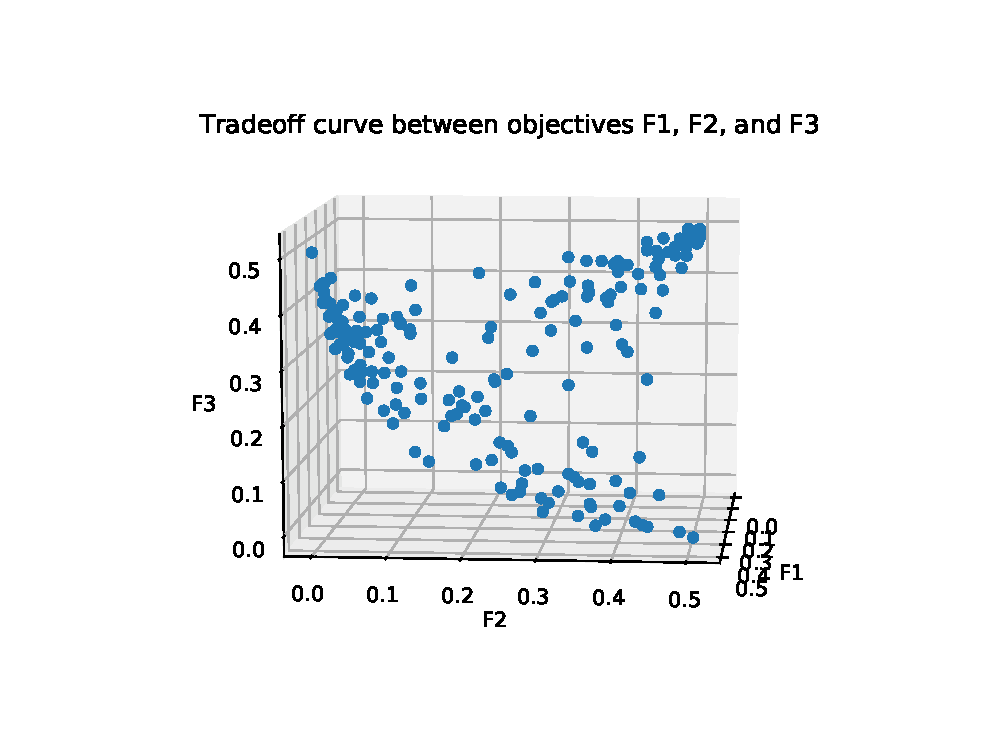
\includegraphics[width=\textwidth]{f_conv_2.eps}
\end{column}
\begin{column}{.48\textwidth}
\begin{itemize}
\item {\tt DTLZ2} from Deb et al.
\item Concave Pareto front $\Rightarrow$ ``harder'' problem
\end{itemize}
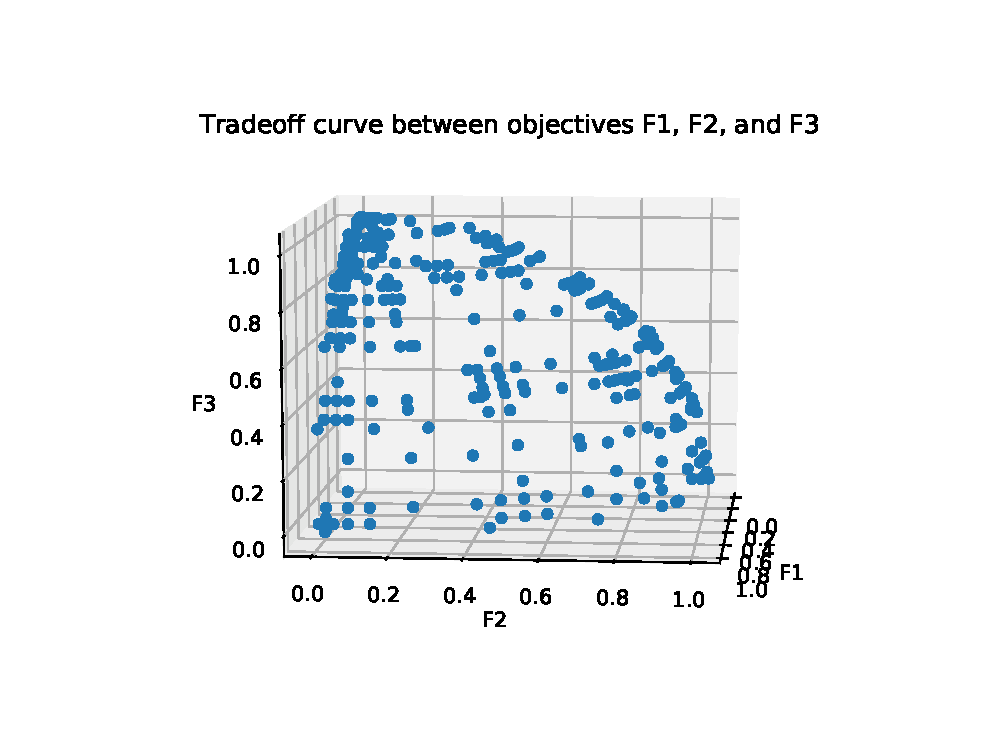
\includegraphics[width=\textwidth]{dtlz2_2.eps}
\end{column}
\end{columns}
\end{frame}
% Performance results
\begin{frame}{Approximation results}
Number of solutions, RMSE, and Delaunay discrepancy (respectively)
for $F_c$ and {\tt DTLZ2}, after a budget of 2000 function evaluations,
with $d=5$ (Averaged over 5 runs).\\
\medskip
Performance metrics:
\begin{enumerate}
\item the {\it cardinality} of the solution set (num pts)
\item the {\it convergence} of the solution points to the true Pareto front (RMSE)
\item the {\it relative spacing/coverage} of the solution set (Delaunay discrep)
\end{enumerate}
\begin{center}
{\tiny
\begin{tabular}{c|ccc}
Prob/Meth&$p=2$&$p=3$&$p=4$\\
\hline
{$F_c$ / {\tt bVTdir}} & 73, .00100, .207 & 173, .0505, .579 & 288, .101, NA\\
{$F_c$ / {\tt libE}} & 78, .0127, .158 & 189, .0560, .429 & 283, .104, .551\\
{{\tt DTLZ2} / {\tt bVTdir}} & 139, .00713, .109 & 354, .0401, .230 & 658, .0443, NA\\
{{\tt DTLZ2} / {\tt libE}} & 66, .103, .201 & 258, .175, .691 & 548, .201, .793\\
\end{tabular}
}
\end{center}
\end{frame}
% Runtimes
\begin{frame}{Runtime performance}
Runtimes for {\tt VTMOP} with 2000 function evaluations (either 1 second or
in range [0.5 s, 1.5 s]), for {\tt bVTdirect} and {\tt libEnsemble}
with $d=5$. Shows CPU time / wall time in seconds, for 36 core machine.\\
\bigskip
\begin{center}
{\tiny
\begin{tabular}{cc|cccc}
$p$ & Method & $F_c$, no var & $F_c$, w/ var & {\tt DTLZ2}, no var
& {\tt DTLZ2}, w/ var\\
\hline
$2$ & {\tt bVTdir} & 2008 / 1037 & 2007 / 1039 & 2007 / 1093 & 2004 / 1082\\
%& {\tt bVTdir2} & NA / 170 & NA / 239 & NA / 175 & NA / 240\\
& {\tt libE} & 2051 / 112 & 2070 / 142 & 2060 / 111 & 2064 / 143\\
\hline
 $3$ & {\tt bVTdir} & 2012 / 717 & 2012 / 719 & 2021 / 797 & 2018 / 797\\
%& {\tt bVTdir2} & NA / 137 & NA / 207 & NA / 165 & NA / 237\\
& {\tt libE} & 2077 / 133 & 2066 / 144 & 2054 / 99 & 2057 / 126\\
\hline
$4$ &{\tt bVTdir} & 2026 / 582 & 2029 / 586 & 2177 / 807 & 2149 / 782\\
%$4$ & {\tt bVTdir2} & NA / 134 & NA / 208 & NA / 280 & NA / 348\\
&{\tt libE} & 2134 / 190 & 2124 / 186 & 2182 / 227 & 2185 / 257\\
\end{tabular}
}
\end{center}
\bigskip
\end{frame}
% Applications and future work
\subsection{Future work}
% Problem difficulties
\begin{frame}{Spectrum of blackbox problems}
Computationally cheap $\xrightarrow{\hspace*{4cm}}$ expensive
\bigskip
\begin{columns}
\begin{column}{.33\textwidth}
\begin{itemize}
\item Eval: $\approx 1$ sec
\item Budget: $\approx 10,000$
\item Software: {\tt NSGA-II}
\end{itemize}
\end{column}
\begin{column}{.33\textwidth}
\begin{itemize}
\item Eval: $\approx 1$ min
\item Budget: $\approx 1000$
\item Software: {\tt VTMOP}
\end{itemize}
\end{column}
\begin{column}{.33\textwidth}
\begin{itemize}
\item Eval: $\approx 1$ hr
\item Budget $\approx 100$ (at most)
\item Software: {\tt FUN3D}? {\tt NASTRAN}?
\pause
\item {\bf Future work!}
\end{itemize}
\end{column}
\end{columns}
\end{frame}
% CV slide
\begin{frame}{Significant work}
\begin{columns}
\begin{column}{.48\textwidth}
\textbf{Peer-Reviewed:}\\
\smallskip
{\tiny
{\it T. H. Chang, et al. ``Least-squares solutions to polynomial systems of
equations with quantum annealing.'' Springer, QINP 18:374 (2019).}\\
\medskip
{\it T. H. Chang, et al. ``Computing the umbrella neighbourhood of a vertex in
the Delaunay triangulation and a single Voronoi cell in arbitrary dimension.''
In IEEE SoutheastCon 2018.}\\
\medskip
{\it T. H. Chang, et al. 
``A polynomial time algorithm for multivariate interpolation in arbitrary
dimension via the Delaunay triangulation.''
In the ACMSE 2018 Conf.}\\
\medskip
{\it T. H. Chang, et al.
``Predicting system performance by interpolation using a high-dimensional Delaunay triangulation.''
In SpringSim 2018, 26th HPC Symp.}\\
}

\textbf{Under Review:}\\
\smallskip
{\tiny
{\it T. H. Chang, et al.
``Algorithm XXX: DELAUNAYSPARSE: Interpolation via a sparse subset of the
Delaunay triangulation in medium to high dimensions.''
Submitted to ACM TOMS (2019).}\\
\medskip
{\it T. H. Chang, et al.
``Managing computationally expensive blackbox multiobjective optimization
problems with libEnsemble.''
Submitted to SpringSim 2020, 28th HPC Symp.}\\
}
\end{column}
\begin{column}{.48\textwidth}
\textbf{Major Awards:}\\
{\small Cunningham Fellow. Virginia Tech, Grad School. 2016--Present}\\
\medskip
{\small SCGSR award. DOE, Office of Sci. Jun--Dec, 2019}\\
\medskip
{\small Various CS/Eng. dept. fellowships. Virginia Tech. 2016--Present}\\
\medskip
\textbf{Projects:}\\
{\small VarSys project at Virginia Tech. NSF grant \#1565314}\\
\medskip
\textbf{Professional:}\\
{\small Reviewer for {\it IEEE SoutheastCon} and {\it JMLR}}
\end{column}
\end{columns}
\end{frame}
\end{document}
